% ============================================================================
% Chapter 1 · Introduction
% Style: no em dashes; concrete hook; funnel from stakes to gap to questions;
% state the gap, the contributions, the scope, and the roadmap explicitly.
% Cross-chapter references use plain "Chapter N" (thesis convention).
% ============================================================================

\section{Introduction}\label{sec:introduction}

In 2024, German day-ahead electricity prices fell below zero for 459 hours,
roughly three times the count of two years earlier
\cite{FfE2025_GermanElectricityPricesEPEX2024}. That is the structural
signature of wind at scale: the more of it a power system absorbs, the less each
additional unit earns on the wholesale market. That tension, between the ambition to build offshore wind and the
economics that erode its value as it is built, is the subject of this thesis.

A wind farm sells its electricity at the price prevailing in the hours it
happens to generate, and because wind output is correlated across a region,
those are precisely the hours in which farms produce together and depress the
price they all receive. What a farm earns per unit of electricity is therefore
the average price of its own generating hours, which sits below the market's
overall average. The fraction of the average price a farm captures in this way
is its capture value, and it declines as regional wind capacity grows, a
process called cannibalisation \cite{Hirth2013}. Because revenue is output
multiplied by the price that output sells at, capture value is increasingly
the term that decides whether an offshore project is viable.

Europe ended 2024 with roughly 36~GW of offshore wind
\cite{Colaluce2025_EuropeOffshoreWind} and plans on the order of 360~GW by 2050
\cite{EuropeanCommission2021_EUReferenceScenario2020}, a tenfold expansion
within the lifetime of a single project. Most of today's capacity
sits in the mature North Sea, where Germany alone operates 9.2~GW
\cite{OffshoreWIND2025_GermanyOffshoreCapacity}; the next wave moves east into the
enclosed Baltic, where the Marienborg Declaration targets 19.6~GW by 2030 against
a technical potential of up to 93~GW \cite{BalticWind2024_BEMIPOffshorePriorities}.
The question is no longer whether offshore wind expands, but where it
expands and what value survives once it does.

Policy makes that question more urgent: REPowerEU lifted the EU's 2030 renewable
target to 42.5\% \cite{REPowerEU2022}, the IEA and IRENA project a tripling
of global renewable capacity by 2030 \cite{IEA2024, IRENA2024}, the Draghi
report names European electricity prices a threat to industrial survival
\cite{Draghi2024}, and the 2024 market reform made the two-sided contract for
difference the default for supported capacity \cite{EUMarketReform2024}.
Each of these forces more zero-marginal-cost generation into the market, and
so deepens the erosion this thesis measures.

Yet the basin where the next wave will land has never been systematically compared
with the North Sea on the metric that decides its viability. Cannibalisation has
been quantified nationally \cite{Hirth2013} and pan-European in aggregate
\cite{Stiewe2025}, but the statistical models used absorb each market's character
into a single fitted constant. They establish that markets differ while leaving
the reason inside that constant, and they cannot be carried into a future in
which the characteristics they absorb have changed. And because investment horizons force projection, every projected capture
value in the literature rests on a single model family never validated
against another. The enclosed Baltic, earlier on its cannibalisation curve
and structurally less able to export its surplus, is the case these gaps
leave unanswered.

This thesis measures and projects the market value of offshore wind across the
open North Sea and the enclosed Baltic, entirely on open data. It asks how the
two basins compare today and how they diverge as the committed buildout is
delivered, what sets the rate at which value is lost and how much of that loss
system design can remove, and whether a model fitted to historical observation
can describe a future lying outside it or whether a model of the power system is
required. Section~\ref{sec:research_gap} states these three questions formally,
after setting out the gaps they follow from.

Answering them requires two models, because no single one can both measure the
present credibly and describe a future that has never occurred. A regression
model fitted to eight years of observed prices measures the present. A system
model, PyPSA-Eur (Python for Power System Analysis), rebuilds the market from
generation costs and the physical network and projects beyond the observed
record. Both are compared against observed capture value wherever it exists, and
that comparison decides which model is used for what
(Section~\ref{sec:design}).

On this design the thesis makes four contributions, the first of which is a
systematic North-Sea-versus-Baltic capture-value comparison at the bidding-zone
resolution where prices form, carried from today's measurement to the 2040
buildout. The
second sets the two models against observation and against each other on the
same quantity, and determines from measurement, rather than by assumption, at which point the projection should pass from one model to the other: the regression model is shown to stop answering where it cannot
extrapolate, the remaining gap is decomposed into the construction steps that
produce it, and the system model's congestion bias is corrected against
observation. The third decomposes the erosion twice, into the structural part no
grid can remove and the congestion part an optimal grid does, and into the
shares of the loss borne by the farm and by the state under the contracts that
now dominate support. The fourth folds capture value into levelised cost to give
a value-adjusted cost of energy per location, and carries it to the decision it
changes, which is where to build. The whole chain rests on open data and open
code, so every number in the thesis can be reproduced.

The study covers both basins through 31 offshore wind farms, sixteen in the North
Sea and fifteen in the Baltic, measured hourly over 2017 to 2024 and projected to
2030 and 2040 under the official European transmission-planning scenarios. The
fourteen countries bordering the two seas hold 21.1~GW of Europe's offshore
capacity today, the remainder sitting mostly in Great Britain, which lies outside
the modelled area. Figure~\ref{fig:study_farms} maps the farms.

\begin{figure}[!htb]
    \centering
    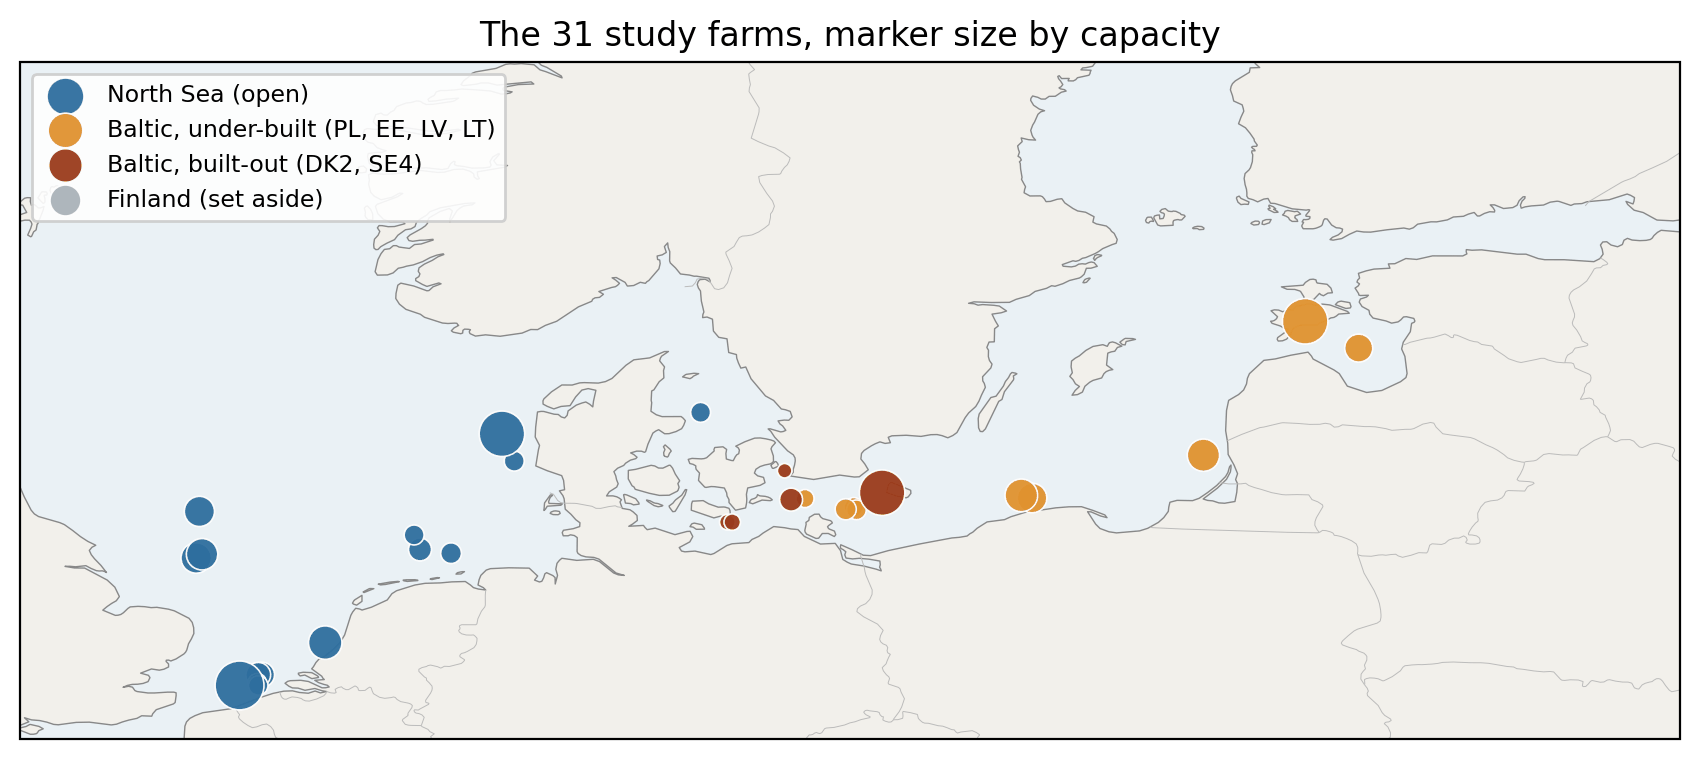
\includegraphics[width=0.92\textwidth]{fig_study_farms}
    \caption{The 31 study farms across the two basins. Marker size is
    proportional to capacity, and the farms are grouped into the four categories
    used throughout the thesis: the open North Sea fleet, the under-built Baltic
    fleet whose buildout is projected here, the built-out zones DK2 and SE4, and
    Finland, which is set aside.}
    \label{fig:study_farms}
\end{figure}
Chapter 2 builds the concepts from first principles and locates the gaps the
questions above fill. Chapter 3 develops the two models and how they are compared. Chapter 4 measures today's value, tests the two models against
observation and against each other, projects the buildout, explains what drives
the erosion, and turns the result into decisions: a break-even price per site
and a ranking of where to build. The accounting of who bears the loss is
carried in Appendix~\ref{app:portfolio}. Chapter 5 answers the three research
questions against that evidence, sets the answers against the literature, and
states the limits of the work. Chapter 6 concludes. The finding that
carries through every chapter is that cannibalisation in the Baltic is a
consequence of the system built around the basin.
